%\documentstyle[epsf,twocolumn]{jarticle}       %LaTeX2e仕様
\documentclass[twocolumn]{jarticle}     %pLaTeX2e仕様(platex.exeの場合)
%\documentclass[twocolumn]{ujarticle}     %pLaTeX2e仕様(uplatex.exeの場合)
%%%%%%%%%%%%%%%%%%%%%%%%%%%%%%%%%%%%%%%%%%%%%%%%%%%%%%%%%%%%%%
%%
%%  基本バージョン
%%
%%%%%%%%%%%%%%%%%%%%%%%%%%%%%%%%%%%%%%%%%%%%%%%%%%%%%%%%%%%%%%%%
\setlength{\topmargin}{-45pt}
%\setlength{\oddsidemargin}{0cm} 
\setlength{\oddsidemargin}{-7.5mm}
%\setlength{\evensidemargin}{0cm} 
\setlength{\textheight}{24.1cm}
%setlength{\textheight}{25cm} 
\setlength{\textwidth}{17.4cm}
%\setlength{\textwidth}{172mm} 
\setlength{\columnsep}{11mm}

\kanjiskip=.07zw plus.5pt minus.5pt


% 【節が変わるごとに (1.1)(1.2) … (2.1)(2.2) と数式番号をつけるとき】
%\makeatletter
%\renewcommand{\theequation}{%
%\thesection.\arabic{equation}} %\@addtoreset{equation}{section}
%\makeatother

%\renewcommand{\arraystretch}{0.95} 行間の設定

%%%%%%%%%%%%%%%%%%%%%%%%%%%%%%%%%%%%%%%%%%%%%%%%%%%%%%%%
\usepackage[dvipdfmx]{graphicx}   %pLaTeX2e仕様(\documentstyle ->\documentclass)\documentclass[dvipdfmx]{graphicx}
\usepackage[dvipdfmx]{color}
\usepackage[subrefformat=parens]{subcaption}
\usepackage{colortbl}
\usepackage{multicol}
%%%%%%%%%%%%%%%%%%%%%%%%%%%%%%%%%%%%%%%%%%%%%%%%%%%%%%%%

\begin{document}

\twocolumn[
\noindent

\hspace{1em}
2021年01月15日
\hfill
\ \ 細川 岳大

\vspace{2mm}

\hrule

\begin{center}
{\Large \bf 進捗報告}
\end{center}
\hrule
\vspace{3mm}
]

% ‚ここから 文章 Start!

\section{今週やったこと}

\begin{itemize}
	\item GAの実験
\end{itemize}

\section{GAの実験}
\subsection{遺伝子}
画像変換は\{AutoContrast, Brightness, Color, Contrast, Equalize, Identity, Posterize, Rotate, Sharpness, ShearX/Y, Solarize, TranslateX/Y\}の14種(一つは恒等変換)を用い,各遺伝子はその遺伝子座に対する変換を用いるかいなかについて0/1の値を持つビットエンコーディングとした.また,\ FixMatch\ における弱及び強変換に対し持つので遺伝子長は28とした.

選択はサイズ2のトーナメント選択,交叉には一様交叉,突然変異は遺伝子座ごとに対立遺伝子に置換されるように設定した.

表\ref{tb:GApara},\ref{tb:FTXpara1},\ref{tb:FTXpara2}に実験の設定を示す.

また得られた個体について全世代における上位10個体を用いて学習した.
\subsection{結果}
図\ref{fig:ex1_1},\ref{fig:ex2_1}に適応度の推移を,
図\ref{fig:ex1_2},\ref{fig:ex2_2}最終個体における各\ transform\ の累積を示す.
実験1,2間で選択されたtrnasformにかなり差異があることから初期収束が起こっている可能性がある.

また表\ref{tb:test}テストに対する識別率を示す.
今回得られたものでは最初期のiterationでは従来のものに勝っているが,
iterationが増えるにつれ逆転するような結果となった.
原因として得られた個体についてweakとstrongをペアとして扱わずバラバラに適用していたことと
時間短縮のために非常に短いみてにおける適応度しか見ていないことが挙げられる.

\begin{table}[h]
	\centering
	\caption{テスト識別率\label{tb:test}}
	\scalebox{1.0}{
		\begin{tabular}{|c|c|c|} \hline
			\multicolumn{3}{|c|}{実験1}\\ \hline
			iteration&従来&今回\\ \hline
			6000&0.241&0.420\\ \hline
			10000&0.261&0.185\\ \hline
			\multicolumn{3}{|c|}{実験2}\\ \hline
			iteration&従来&今回\\ \hline
			10000&0.314&0.409\\ \hline
			15000&0.634&0.435\\ \hline
		\end{tabular}
	}
\end{table}

\begin{figure}[h]
	\begin{center}
		\vspace*{3mm}
		\hspace*{-12mm}
		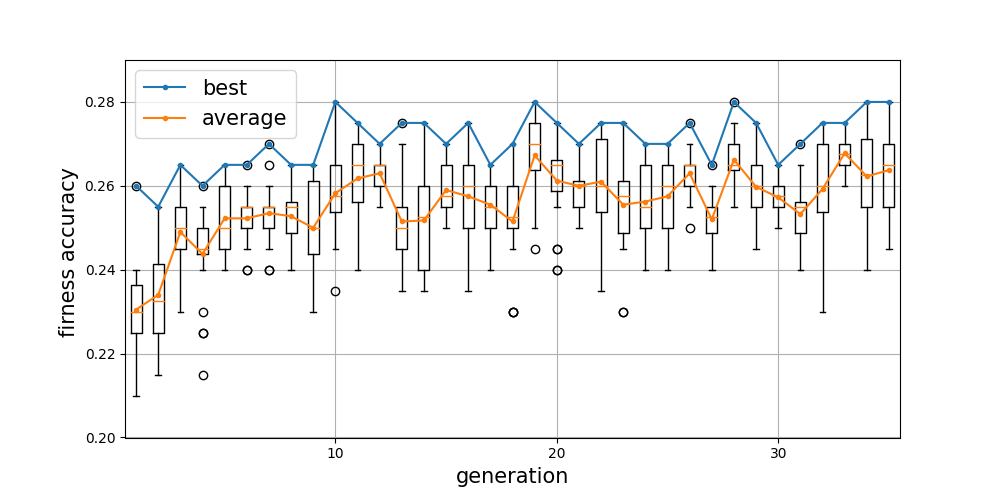
\includegraphics[height=65mm,width=90mm]{graph1_1.png}
		\caption{実験1の適応度\label{fig:ex1_1}}
	\end{center}
\end{figure}

\begin{figure}[h]
	\begin{center}
		\vspace*{3mm}
		\hspace*{-12mm}
		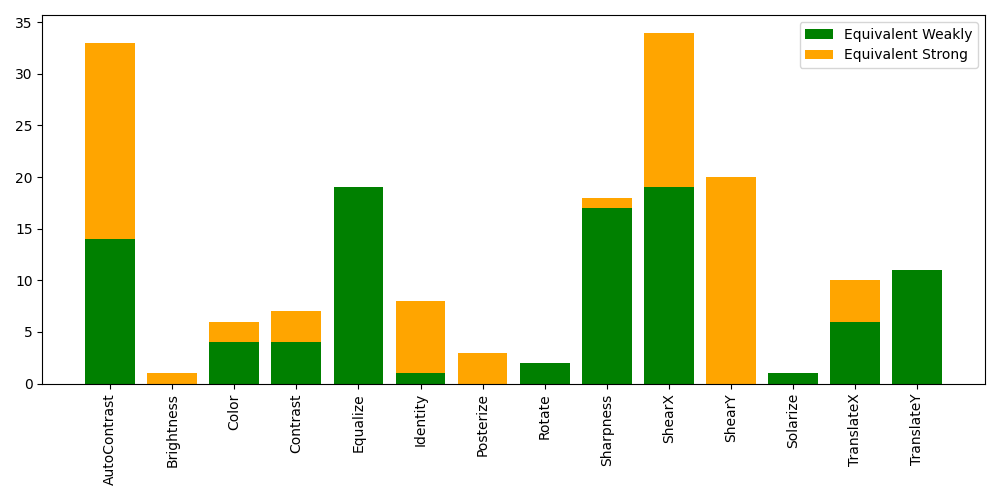
\includegraphics[height=60mm,width=90mm]{graph1_2.png}
		\caption{実験1の最終個体\label{fig:ex1_2}}
	\end{center}
\end{figure}

\begin{figure}[h]
	\begin{center}
		\vspace*{-3mm}
		\hspace*{-12mm}
		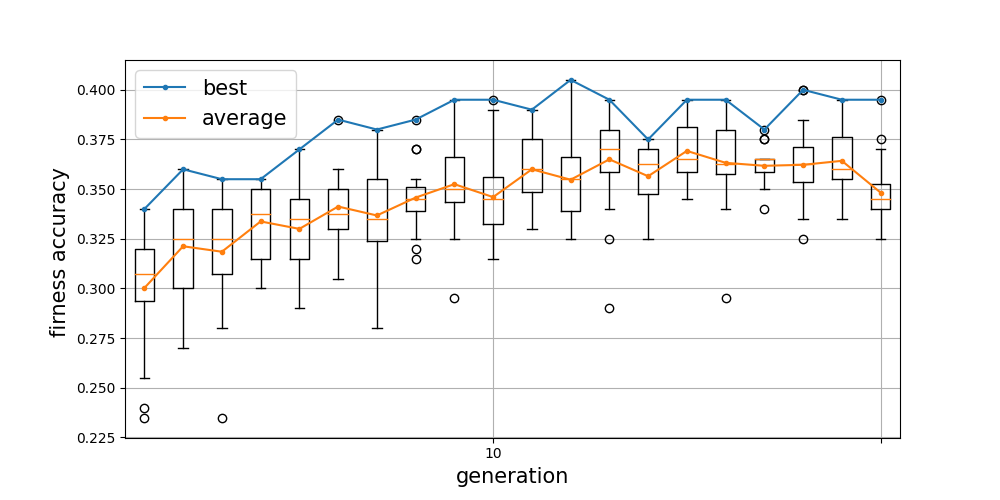
\includegraphics[height=65mm,width=90mm]{graph2_1.png}
		\caption{実験2の適応度\label{fig:ex2_1}}
	\end{center}
\end{figure}

\begin{figure}[h]
	\begin{center}
		\vspace*{-3mm}
		\hspace*{-12mm}
		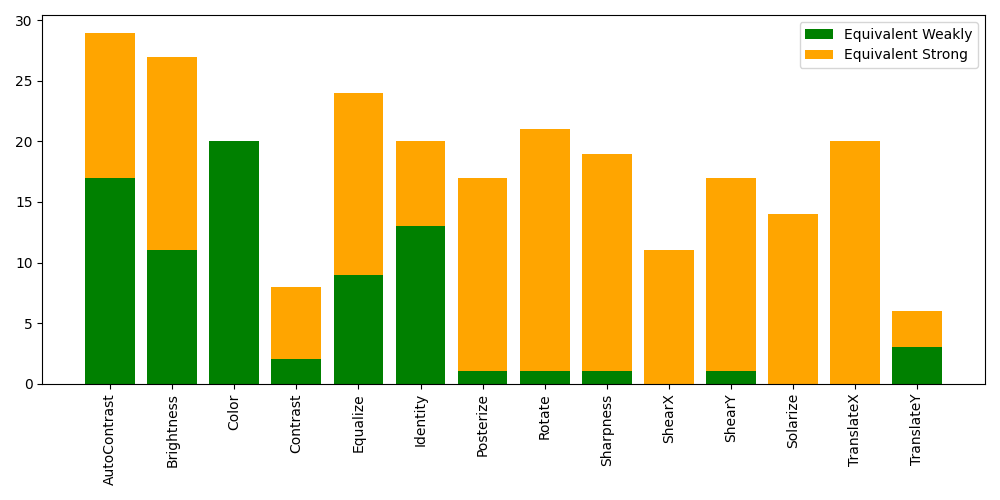
\includegraphics[height=60mm,width=90mm]{graph2_2.png}
		\caption{実験2の最終個体\label{fig:ex2_2}}
	\end{center}
\end{figure}



\section{来週の課題}
\begin{itemize}
	\item 実験設定の改良
	\item SimCLRを用いた実験
\end{itemize}


\begin{table}[t]
	\centering
	\caption{GAの設定\label{tb:GApara}}
	\scalebox{1.0}{
		\begin{tabular}{|c||c|} \hline
			個体数&20\\ \hline
			交叉率&1.0\\ \hline
			突然変異率&0.03\\ \hline
		\end{tabular}
	}
\end{table}

\begin{table}[h]
	\centering
	\caption{実験1の設定\label{tb:FTXpara1}}
	\scalebox{1.0}{
		\begin{tabular}{|c|c|c|} \hline
			model&\multicolumn{2}{c|}{WideResNet16-2}\\ \hline\hline
			data set&\multicolumn{2}{c|}{cifar10}\\ \hline
			train&labeled&50\\ \cline{2-3}
			&unlabeled&49750\\ \hline
			valid&\multicolumn{2}{|c|}{200}\\ \hline
			test&\multicolumn{2}{|c|}{10000}\\ \hline\hline
			\multicolumn{3}{|c|}{事前学習}\\ \hline
			batch size&labeled&32\\ \cline{2-3}
			&unlabeled&$32*7$\\ \hline
			augment&labeled&RandAugment\\ \cline{2-3}
			&weak&Identity\\ \cline{2-3}
			&strong&Identity\\ \hline
			optimizer&\multicolumn{2}{c|}{SGD(lr=0.05,momntum=0.9)}\\ \hline
			num\_iterations&\multicolumn{2}{c|}{5000}\\ \hline\hline
			\multicolumn{3}{|c|}{GAの評価}\\ \hline
			batch size&labeled&16\\ \cline{2-3}
			&unlabeled&$16*3$\\ \hline
			augment&labeled&RandAugment\\ \hline
			num\_iterations&\multicolumn{2}{c|}{1000}\\ \hline
		\end{tabular}
	}
\end{table}

\begin{table}[h]
	\centering
	\caption{実験2の設定\label{tb:FTXpara2}}
	\scalebox{1.0}{
		\begin{tabular}{|c|c|c|} \hline
			model&\multicolumn{2}{c|}{WideResNet16-2}\\ \hline\hline
			data set&\multicolumn{2}{c|}{cifar10}\\ \hline
			train&labeled&50\\ \cline{2-3}
			&unlabeled&49750\\ \hline
			valid&\multicolumn{2}{|c|}{200}\\ \hline
			test&\multicolumn{2}{|c|}{10000}\\ \hline\hline
			\multicolumn{3}{|c|}{事前学習}\\ \hline
			batch size&labeled&32\\ \cline{2-3}
			&unlabeled&$32*7$\\ \hline
			augment&labeled&RandAugment\\ \cline{2-3}
			&weak&Identity\\ \cline{2-3}
			&strong&Identity\\ \hline
			optimizer&\multicolumn{2}{c|}{SGD(lr=0.05,momntum=0.9)}\\ \hline
			num\_iterations&\multicolumn{2}{c|}{20000}\\ \hline\hline
			\multicolumn{3}{|c|}{GAの評価}\\ \hline
			batch size&labeled&16\\ \cline{2-3}
			&unlabeled&$16*2$\\ \hline
			augment&labeled&RandAugment\\ \hline
			num\_iterations&\multicolumn{2}{c|}{3000}\\ \hline
		\end{tabular}
	}
\end{table}



\end{document}


